\documentclass{standalone}
\usepackage{graphicx}	
\usepackage{amssymb, amsmath}
\usepackage{color}
\usepackage{wasysym}

\usepackage{tikz}
\usetikzlibrary{intersections, backgrounds}
\usepackage{pgfmath}

\definecolor{light}{RGB}{220, 188, 188}
\definecolor{mid}{RGB}{185, 124, 124}
\definecolor{dark}{RGB}{143, 39, 39}
\definecolor{highlight}{RGB}{180, 31, 180}
\definecolor{gray10}{gray}{0.1}
\definecolor{gray20}{gray}{0.2}
\definecolor{gray30}{gray}{0.3}
\definecolor{gray40}{gray}{0.4}
\definecolor{gray60}{gray}{0.6}
\definecolor{gray70}{gray}{0.7}
\definecolor{gray80}{gray}{0.8}
\definecolor{gray90}{gray}{0.9}
\definecolor{gray95}{gray}{0.95}

\newcommand*{\offset}{0.025}

\begin{document}

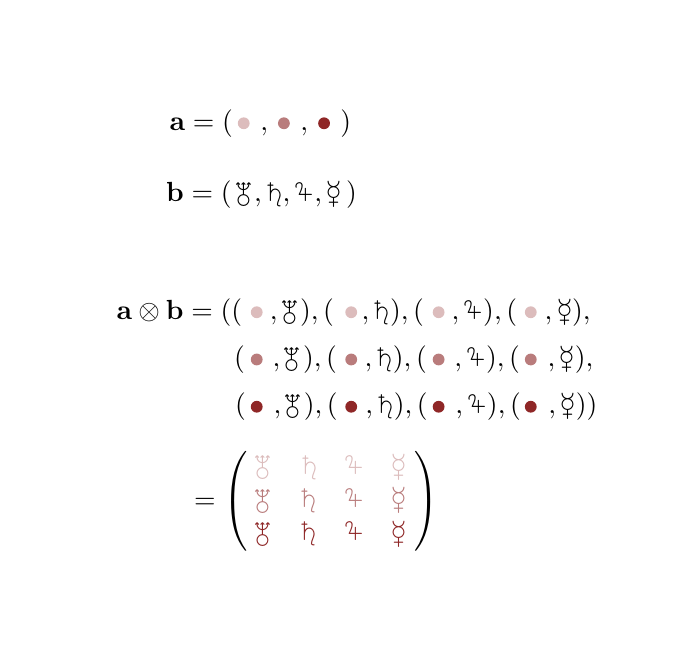
\begin{tikzpicture}[scale=0.3, thick]

\pgfmathsetmacro{\cx}{2}
\pgfmathsetmacro{\cy}{3}

\draw[white] (-10, -16) rectangle (17, 9);

\node[align=left] at (0, 5) { $\mathbf{a} = ( \quad, \quad, \quad )$ };
\fill[light] (-0.9, 5) circle (0.25);
\fill[mid] (0.8, 5) circle (0.25);
\fill[dark] (2.5, 5) circle (0.25);

\node[align=left] at (0.05, 2) { $\mathbf{b} = ( \, \neptune, \saturn, \jupiter, \mercury \, )$ };

\node[] at (3.75, -3) 
{ $\mathbf{a} \otimes \mathbf{b} = ( (\quad, \neptune), (\quad, \saturn), (\quad, \jupiter), (\quad, \mercury), $ };
\fill[light] (-4.1 + 3.75, -3) circle (0.25);
\fill[light] (-0.1 + 3.75, -3) circle (0.25);
\fill[light] (3.6 + 3.75, -3) circle (0.25);
\fill[light] (7.5 + 3.75, -3) circle (0.25);

\node[] at (2.55 + 3.75, -5) 
{ $(\quad, \neptune), (\quad, \saturn), (\quad, \jupiter), (\quad, \mercury), $ };
\fill[mid] (-4.1 + 3.75, -5) circle (0.25);
\fill[mid] (-0.1 + 3.75, -5) circle (0.25);
\fill[mid] (3.6 + 3.75, -5) circle (0.25);
\fill[mid] (7.5 + 3.75, -5) circle (0.25);

\node[] at (2.65 + 3.75, -7) 
{ $(\quad, \neptune), (\quad, \saturn), (\quad, \jupiter), (\quad, \mercury) )$ };
\fill[dark] (-4.1 + 3.75, -7) circle (0.25);
\fill[dark] (-0.1 + 3.75, -7) circle (0.25);
\fill[dark] (3.6 + 3.75, -7) circle (0.25);
\fill[dark] (7.5 + 3.75, -7) circle (0.25);


\node[] at (0.6, -11) 
{ $\mathbf{a} \otimes \mathbf{b} =
\begin{pmatrix}
\; \neptune & \saturn & \jupiter & \mercury \; \\
\; \neptune & \saturn & \jupiter & \mercury \; \\
\; \neptune & \saturn & \jupiter & \mercury \;
\end{pmatrix} $ };

\fill[white] (-7, -12) rectangle (-3, -10);
\fill[white] (-0.7, -13.5) rectangle (6.2, -8.5);

\node[light] at (-0.03, -9.59 + 0.01) { $\neptune$ };
\node[light] at (1.86575, -9.59 + 0.005) { $\saturn$ };
\node[light] at (3.79, -9.59 + 0.115) { $\jupiter$ };
\node[light] at (5.69, -9.59 + 0.04) { $\mercury$ };

\node[mid] at (-0.03, -11 + 0.01) { $\neptune$ };
\node[mid] at (1.865, -11 + 0.01) { $\saturn$ };
\node[mid] at (3.79, -11 + 0.12) { $\jupiter$ };
\node[mid] at (5.69, -11 + 0.04) { $\mercury$ };

\node[dark] at (-0.03, -12.4 + 0.01) { $\neptune$ };
\node[dark] at (1.865, -12.4 + 0.01) { $\saturn$ };
\node[dark] at (3.79, -12.4 + 0.12) { $\jupiter$ };
\node[dark] at (5.69, -12.4 + 0.04) { $\mercury$ };

\end{tikzpicture}

\end{document}  